\section{Group Theory}

The study of modern abstract algebra begins with the simple abstract definition of a \hlt{group}, and quickly builds up complexity with structures of such objects. It is useful to isolate specific characteristics and the structure imposed on an object sharing similar characteristics. The structure of the algebraic object, made more precise with the concept of isomorphism, is used repeatedly in the study of groups.

\subsection{Introduction to Groups}

The basic algebraic structure to be studied in Group Theory is introduced in this subsection.

\subsubsection{Basic Axioms}

\begin{definition}{\color{white}space}
\begin{enumerate}[label=(\roman*)]
\setlength{\itemsep}{0pt}
\item A \hlt{binary operation} $*$ on a set $G$ is a function $*: G \times G \rightarrow G$. For any $a,b \in G$, write $a * b$ for $*(a,b)$.
\item A binary operation $*$ on a set $G$ is \hlt{associative} if $\forall a,b,c \in G$, $(a*b)*c = a*(b*c)$
\item If $*$ is a binary operation on a set $G$, then $a,b \in G$ \hlt{commutes} if $a*b = b*a$. Then $*$ (or $G$) is commutative if $\forall a,b,\in G, a*b = b*a$.
\item For $H \subseteq G$, the restriction of $*$ to $H$ is a binary operation on $H$, i.e., $\forall a,b, \in H, a*b \in H$. \\
    $H$ is \hlt{closed} under $*$.
\end{enumerate}
\end{definition}

The examples of operations are as follows.

\begin{example}{\color{white}space}
\begin{enumerate}[label=(\roman*)]
\setlength{\itemsep}{0pt}
\item $+$ (addition) is a commutative binary operation on $\Z, \Q, \R, \C$.
\item $\times$ (multiplication) is a commutative binary operation on $\Z, \Q, \R, \C$.
\item $-$ (subtraction) is a non-commutative binary operation on $\Z$, where $-(a,b)=a-b $. The map $a \rightarrow -a$ is not a binary opeartion.
\item $-$ (subtraction) is not a binary operation on $\Z^+, \Q^+, \R^+$. If $a<b$, then $a-b \notin \Z^+, \Q^+, \R^+$.
\item Vector cross product of two vectors is a binary operation which is neither associative nor commutative.
\end{enumerate}
\end{example}

We then have the following definition of groups.

\begin{definition}
\label{def:group}
A \hlt{group} is an ordered pair $(G,*)$ where $G$ is a set, and $*$ is a binary operation on $G$ satisfying the following exaioms:
\begin{enumerate}[label=(\roman*)]
\setlength{\itemsep}{0pt}
\item Associativity: $(a*b)*c = a*(b*c)$ $\forall a,b,c, \in G$
\item Existence of identity: $e \in G$ such that $\forall a\in G$, we have $a*e = e*a = a$
\item Existence of inverse: $a^{-1} \in G$ such that $\forall a\in G$, we have $a*a^{-1} = a^{-1}a = e$
\end{enumerate}
The group is \hlt{abelian} if $a*b = b*a$ $\forall a,b, \in G$.
The group is a \hlt{finite group} if $G$ is a finite set. \\
Axiom (ii) ensures a group is always nonempty. 
\end{definition}

\begin{example}{\color{white}space}
\begin{enumerate}[label=(\roman*)]
\setlength{\itemsep}{0pt}
\item The basic groups are $(\Z, +), (\Q, +), (\R, +), (\C, +)$ with $e=0$ and $a^{-1} = -a$ $\forall a$
\item The multiplicative groups are $(\Q - \{0\}, \times), (\R- \{0\}, \times), (\C- \{0\}, \times), (\Q^+, \times), (\R^+, \times)$ with $e=1$ and $a^{-1} = \frac{1}{a}$. Note that $(\Z - \{0\}, \times)$ is not a group as the element $2$ (for instance) does not have an inverse
\item The additive group consisting of vector space $V$, i.e., $(V,+)$
\item For $n \in \Z^+$, $(\Z / n\Z, +)$ is an abelian group. The identity is $e=\overline{0}$ $\forall \overline{a} \in \Z / n\Z$. The inverse of $\overline{a}$ is $\overline{-a}$. Hence the group operation is addition of classes$\mod{n}$
\item For $n \in \Z^+$, $((\Z / n\Z)^{\times}, \times)$ of equivalence classes $\overline{a}$ which have multiplicative inverses$\mod{n}$ is an abelian group under multiplication of residue classes. The identity is $e=\overline{1}$. By definition of $(\Z / n\Z)^{\times}$, each element has a multiplicative inverse. Group operation is multiplication of classes$\mod{n}$. 
\end{enumerate}
\end{example}

\begin{definition}
If $(A, *)$ and $(B,\diamond)$ are groups, then we can from new group $A \times B$, which is the \hlt{direct product}, with elements are in Cartesian product $A \times B = \{(a,b) \ | \ a\in A, b\in B\}$, with operation defined component-wise: $(a_1, b_1)(a_2, b_2) = (a_1 * a_2, b_1 \diamond b_2)$
\end{definition}

We now prove two basic results that allows discussion of the identity and inverse of an element.

\begin{proposition}
\label{prop:proofgroupop}
If $G$ is a group under operation $*$, then
\begin{enumerate}[label=(\roman*)]
\setlength{\itemsep}{0pt}
\item the identity of $G$ is unique
\item for each $a\in G$, $a^{-1}$ is uniquely determined
\item $(a^{-1})^{-1} = a$ $\forall a\in G$
\item $(a*b)^{-1} = (b^{-1}) * (a^{-1})$
\item for any $a_1, a_2, \ldots, a_n \in G$, the value of $a_1 * a_2 * \cdots a_n$ is independent of how the expression is bracketed (the \hlt{generalised associative law})
\end{enumerate}
\end{proposition}
\begin{proof}{\color{white}space}
\begin{enumerate}[label=(\roman*)]
\setlength{\itemsep}{0pt}
\item If $f, g$ are both identities, then by Definition \ref{def:group}(ii) of a group $f*g = f$ (with $a=f, e=g$). By the same axiom, $f*g = g$ (with $a=g, e=f$). Hence, $f=g=e$, and the identity is unique.
\item Assume $b,c$ are both inverses of $a$, and let $e$ be the identity of $G$. By  Definition \ref{def:group}(iii), $a*b = e$ and $c*a = e$, thus
\begin{align}
c &= c*e &&\textnormal{ (by definition of $e$ in Definition \ref{def:group}(iii))} \nonumber \\ 
& = c * (a*b) &&\textnormal{ (since $e = a*b$)} \nonumber \\
& = (c*a) * b &&\textnormal{ (associative law)} \nonumber \\
& = e*b &&\textnormal{ (since $e = c*a$)} \nonumber \\
& = b &&\textnormal{ (by Definition \ref{def:group}(iii))} \nonumber
\end{align}
\item By part (ii), $a$ has a unique inverse. By definition of $a^{-1}$, with $a$ and $a^{-1}$ interchanged, this shows that $a$ satisfies the defining property for the inverse of $a^{-1}$, hence $a$ is the inverse of $a^{-1}$.
\item Let $c=(a*b)^{-1}$. By definition of $c$, $(a*b)*c = e$. By associative law, $a*(b*c) = e$.\\
Multiply both sides on left by $a^{-1}$ to get $a^{-1}*(a*(b*c)) = a^{-1} * e$.\\
By associative law and definition of $e$, $(a^{-1}) * (b*c) = a^{-1}$, hence $e*(b*c) = a^{-1}$.\\
Thus $b*c = a^{-1}$. Multiply both sides on left by $b^-1$.
\begin{align}
b^{-1} * (b*c) &= b^{-1} * a^{-1} \nonumber \\
(b^{-1} * b)*c) &= b^{-1} * a^{-1} \nonumber \\
e*c &= b^{-1} * a^{-1} \nonumber \\
c &= b^{-1} * a^{-1} \nonumber
\end{align}
\item By induction on $n$. \impt{PROOF NOT COMPLETE. TBD.} \label{wip:proofgroupop}
\end{enumerate}
\end{proof}

We use the notation $ab$ for $a \cdot b$, and identity of an abstract group $G$ as $1$ for brevity.\\
For any group with $\cdot$ operation, $x \in G$ and $n \in \Z^+$, we denote $xx\cdots x$ ($n$ terms) with $x^n$, $x^{-1} x^{-1} \cdots x^{-1}$ ($n$ terms) by $x^{-n}$. The identity of $G$ is then denoted $x^0 = 1$.

\begin{proposition}
Let $G$ be a group, and let $a,b \in G$. The equations $ax=b$ and $ya=b$ have unique solutions for $x,y \in G$. In particular, the left and right cancellation law holds in $G$, i.e.,
\begin{enumerate}[label=(\roman*)]
\setlength{\itemsep}{0pt}
\item if $au=av$ then $u=v$, and
\item if $ub=vb$, then $u=v$
\end{enumerate}
\end{proposition}
\begin{proof}
Solve $ax=b$ by multiplying both sides on left by $a^{-1}$ and simplify to get $x=a^{-1}b$. Uniqueness of $x$ follows as $a^{-1}$ is unique. Similarly, if $ya=b$, then $y=ba^{-1}$. If $au=av$, multiply both sides on left by $a^{-1}$ to get $u=v$. Similarly, the right cancellation law holds.
\end{proof}

A consequence of the proposition is that if $a$ is any element of $G$, and for some $b\in G$, $ab=e$ or $ba=e$, then $b=a^{-1}$, i.e., we do not have to show both equations hold.\\
Also, if for some $b\in G$, $ab=a$ (or $ba=a$), then $b$ must be the identity of $G$. We do not have to check $bx=xb=x$ for all $x\in G$

\begin{definition}
For group $G$ and $x\in G$, the \hlt{order of $x$} is the smallest positive integer $n$ such that $x^n = 1$, denoted $\abs{x}$. If no positive power of $x$ is the identity, then $\abs{x} = \infty$.
\end{definition}

\begin{example}{\color{white}space}
\begin{enumerate}[label=(\roman*)]
\setlength{\itemsep}{0pt}
\item In multiplicative groups $\R - \{0\}$ or $\Q - \{0\}$, the element $-1$ has order $2$, and other non-identity elements have infinite order.
\item In additive groups $\Z, \Q, \R, \C$, every nonzero (non-identity) element has infinite order.
\item The additive group $\Z / 9\Z$'s element $\overline{6}$ has order $3$, $\overline{5}$ has order $9$.
\end{enumerate}
\end{example}

\begin{definition}
Let $G = {g_1, g_2, \ldots, g_n}$ be a finite group with $g_1 = 1$. The \hlt{multiplication table} or \hlt{group table} of $G$ is the $n \times n$ matrix whose $i,j$ entry is the group element $g_i g_j$.
\end{definition}

\subsubsection{Dihedral Groups}

This family of groups consists of elements which are symmetries of geometric objects. First, we introduce the notion of generators and relations as they provide simple ways of describing and computing groups.

\begin{definition}
Any equations in a general group $G$ that generators satisfy are called \hlt{relations} in $G$.\\
If a group $G$ is generated by a subset $S$, and there is some collection of relations, say $R_1, R_2, \ldots, R_m$ (where each $R_i$ is an equation in the elements from $S \cup \{1\}$ such that any relations among the elements of $S$ can be deduced from these, then this is a \hlt{presentation of $G$}, written:
\begin{equation}
G = \langle S \ \vert \ R_1, R_2, \ldots, R_m \rangle \nonumber 
\end{equation}
\end{definition}

Note that in an arbitrary presentation, it may be difficult to tell when two elements of the group are equal. It may not be evident what the order of presented group is, or even whether the group is finite or infinite.\\
Also even in quite simple presentation, some 'collapsing' may occur as relations are intertwined in some unobvious way. There may be 'hidden' or implicit relations that are not explicitly given in the presentation, but rather are the consequences of the specified ones.

\begin{definition}
A \hlt{dihedral group} is the group of symmetries of a regular $n$-gon, denoted
\begin{equation}
D_{2n} = \langle r,s \ \vert \ r^n = s^2 = 1, rs = sr^{-1} \rangle \nonumber
\end{equation}
where $r$ is a rotation counterclockwise about the origin by $\frac{2\pi}{n}$,\\
$s$ is a reflection about the line of symmetry through the vertex $1$
\end{definition}

\begin{figure}[H]
\centering
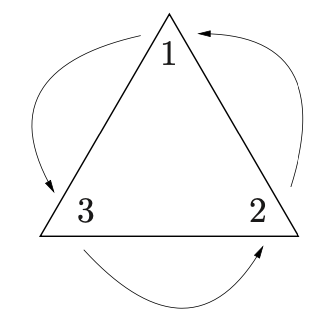
\includegraphics[scale=0.4]{dihedralgroups}
\caption{Example of an equilateral triangle as a Dihedral Group $D_6$}
\end{figure}

\begin{remark}
The properties of dihedral groups are as follows:
\begin{enumerate}[label=(\roman*)]
\setlength{\itemsep}{0pt}
\item $\abs{r}=n$, as $1, r, \ldots, r^n$ are all distint, and $r^n = 1$
\item $\abs{s}=2$, as $s^2 = 1$
\item $s \neq r^i$ for any $i$
\item $sr^i \neq sr^j$ for all $0 \leq i, j \leq n-1$, with $i \neq j$\\
Hence $D_{2n} = \{1,r,r^2,\ldots, r^{n-1}, s, sr, sr^2, \ldots, sr^{n-1}\}$.\\
Each element can be written uniquely in the form $s^k r^i$ for $k \in {0,1}$, $0\leq i \leq n-1$.
\item $rs=sr^{-1}$. Hence $r$ and $s$ do not commute, and $D_{2n}$ is non-abelian.
\item $r^i s = sr^{-i}$ for all $0\leq i \leq n$
\end{enumerate}
\end{remark}

\subsubsection{Symmetric Groups}

\begin{definition}
Let $\Omega$ be any nonempty set, and $S_{\Omega}$ be the set of all bijections from $\Omega$ to itself (the set of all permutations of $\Omega$. Then the set $S_{\Omega}$ is a group under function composition $\circ$.\\
The identity of $S_{\Omega}$ is the permutation $1$ defined by $1(a)=a \ \forall a\in \Omega$.\\
For every permutation $\sigma: \Omega \rightarrow \Omega$ there is a $2$-sided inverse function $\sigma^{-1}: \Omega \rightarrow \Omega$ satisfying $\sigma \circ \sigma^{-1} = \sigma^{-1} \circ \sigma = 1$. Thus all group axioms hold for $(S_{\Omega}, \circ)$, the \hlt{symmetric group on the set $\Omega$}.\\
The elements of $S_{\Omega}$ are the permutations of $\Omega$, not elements of $\Omega$ itself.\\
If $\Omega = \{1,2,\ldots, n\}$ is a finite set, then $S_n$ is the \hlt{symmetric group of degree $n$}.
\end{definition}

The group $S_n$ plays an important role as a means of illustrating and motivating the general theory.

\begin{theorem}
The order of $S_n$ is $n!$.
\end{theorem}
\begin{proof}
The permutations of $\{1,2,\ldots, n\}$ are precisely the injective functions of this set to itself as it is finite. We count the number of injective functions. For $\sigma(n)$, this is precisely $n \cdot (n-1) \cdot (n-2) \cdots 2 \cdot 1 = n!$ possible injective functions from $\{1,2,\ldots, n\}$ to itself.
\end{proof}

We now introduce the notation for writing elements $\sigma$ of $S_n$ with cycle decomposition.

\begin{definition}
A \hlt{cycle} is a string of integers which represents the elements of $S_n$ which cyclically permutes these integers and fixes other integers.\\
The cycle $(a_1 \ a_2 \ \cdots \ a_m)$ is the permutation which sends $a_i$ to $a_{i+1}$, $1 \leq i \leq m-1$ and sends $a_m$ to $a_1$.\\
In general, for each $\sigma \in S_n$, the numbers from $1$ to $n$ will be rearranged and grouped into $k$ cycles of the form
\begin{equation}
(a_1 \ a_2 \ \cdots \ a_{m_1})(a_{m_1 + 1} \ a_{m_1 +2} \ \cdots \ a_{m_2}) \cdots (a_{m_{k-1} + 1} \ a_{m_{k-1} + 2} \ \cdots \ a_{m_k}) \nonumber
\end{equation}
\end{definition}

\begin{remark}
In Cauchy's two line notation, the natural order of elements of $\Omega$, say $x_1, x_2, \ldots, x_n$ is listed in the first row, then the images of each element in the second row.
\begin{equation}
\sigma = 
\begin{pmatrix}
x_1 & x_2 & \cdots & x_n \\
\sigma(x_1) & \sigma(x_2) & \cdots & \sigma(x_n)
\end{pmatrix} \nonumber
\end{equation}
We may omit the first row and write the permutation in one-line notation as:
\begin{equation} 
\begin{pmatrix}
\sigma(x_1) & \sigma(x_2) & \cdots & \sigma(x_n)
\end{pmatrix} \nonumber
\end{equation}
\end{remark}

\begin{definition}
The \hlt{length} of a cycle is the number of integers which appear in it.\\
A cycle of length $t$ is called a \hlt{$t$-cycle}.\\
Two cycles are \hlt{disjoint} if they have no numbers in common.\\
The inverse permutation is given by reversing the order of elements in the permutation's cycles.
\end{definition}

\begin{algorithm}
The \hlt{cycle decomposition algorithm} is as follows:
\begin{enumerate}[label=\arabic*.]
\setlength{\itemsep}{0pt}
\item Write an opening bracket then select an arbitrary element $x$ of $\Omega$ and write it down: $(x$
\item Trace the orbit of $x$, write down its values over successive applications of $\sigma$: $(x \ \sigma(x) \ \sigma(\sigma(x)) \cdots$
\item Repeat until the value returns to $x$ and write a closing parenthesis rather than $x$: $(x \ \sigma(x) \ \sigma(\sigma(x)) \cdots)$
\item Now continue with an element $y$ of $\Omega$ not yet written down, and proceed in the same way: $(x \ \sigma(x) \ \sigma(\sigma(x)) \cdots)(y \cdots)$
\item Repeat until all elements of $\Omega$ are written in cycles.
\end{enumerate}
\end{algorithm}

\subsubsection{Matrix Groups}

Matrix groups have coefficients that come from fields. A field is the smallest mathematical structure which all arithmetic operations $(+, -, \times, \div)$ (division by nonzero elements) can be performed.

\begin{definition}
A \hlt{field} is a set $F$ with two binary operations $+, \cdot$ on $F$ such that $(F, +)$ is an abelian group (with identity $0$), and $(F-\{0\}, \cdot)$ is also an abelian group. The following distributive law holds:
\begin{equation}
a\cdot (b+c) = (a \cdot b) + (a \cdot c), \forall a,b,c \in F \nonumber
\end{equation}
For any field $F$, let $F^{\times} = F - \{0\}$
\end{definition}

\begin{definition}
A \hlt{matrix group} is a group $G$ consisting of invertible matrices over a field $K$, with the operation of matrix multiplication.\\
The \hlt{general linear group} of degree $n$ is the set of $n \times n$ invertible matrices with matrix multiplication, denoted $GL_n(\F)$. If $n \geq 2$, then the group $GL_n(\F)$ is not abelian.\\
The \hlt{special linear group} is a subgroup of $GL_n(\F)$, consisting of matrices with determinant $1$, denoted $SL_n(\F)$.
\end{definition}

We dive deeper into the results in Modules and Vector Spaces in Section \ref{sect:modandvec}.

\subsubsection{The Quaternion Group}

\begin{definition}
The \hlt{quaternion group} is defined by $Q_8 = \{1, -1, i, -i, j, -j, k, -k\}$, with product $\cdot$ computed as follows:
\begin{alignat*}{2}
1 \cdot a &= a \cdot 1 = a &&\forall a \in Q_8 \nonumber \\
(-1) \cdot (-1) = 1,\ \ &(-1) \cdot a = a \cdot (-1) = -a \ \ \ \ &&\forall a \in Q_8 \nonumber \\
i \cdot i &= j \cdot j = k \cdot k= -1 \nonumber \\
i \cdot j &= k, \ \ \ \ \ \ \ j \cdot i = -k \nonumber \\
j \cdot k &= i, \ \ \ \ \ \ \ k \cdot j = -i \nonumber \\
k \cdot i &= j, \ \ \ \ \ \ \ i \cdot k = -j \nonumber
\end{alignat*}
Note that $Q_8$ is a non-abelian group of order 8.
\end{definition}

\begin{figure}[H]
\centering
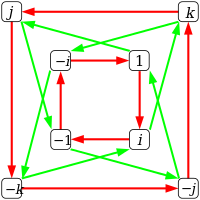
\includegraphics[scale=0.4]{quaterniongroup}
\caption{The Cayley diagram of the Quaternion Group $Q_8$.}
\end{figure}

\subsubsection{Homomorphism and Ismomorphism}

We define what makes two group 'look the same', i.e., having exactly the same group-theoretic structure (an isomorphism) in this section.

\begin{definition}
Let $(G, *), (H, \diamond)$ be groups. A map $\varphi: G \rightarrow H$ such that
\begin{equation}
\varphi(x*y) = \varphi(x) \diamond \varphi(y), \ \ \forall x,y \in G \nonumber
\end{equation}
is a \hlt{homomorphism}.
\end{definition}

If the group operations for $G, H$ are not explicitly written, then this is simply $\varphi(xy) = \varphi(x) \varphi(y)$, but the product $xy$ on the left is computed in $G$, while the product $\varphi(x) \varphi(y)$ is computed in $H$.\\
Intuitively, a map $\varphi$ is a homomorphism if it respects the group structures of its domains and codomains.

\begin{definition}
The map $\varphi: G \rightarrow H$ is a \hlt{isomorphism} and $G$ and $H$ are \hlt{isomorphic}, denoted $G \cong H$, if:
\begin{enumerate}[label=(\roman*)]
\setlength{\itemsep}{0pt}
\item $\varphi$ is a homomorphism (i.e., $\varphi(xy) = \varphi(x) \varphi(y)$), and
\item $\varphi$ is a bijection.
\end{enumerate}
\end{definition}

Intuitively, $G$ and $H$ are the same group, except the elements and operations may be written different in $G$ and $H$. Thus, any property which $G$ has which only depends on group structure of $G$ also holds for $H$.

\begin{definition}
Let $\mathscr{G}$ be any nonempty collection of groups. Then the relation $\cong$ is an equivalent relation on $\mathscr{G}$, and the equivalence classes are called \hlt{isomorphism classes}.
\end{definition}

\begin{example}{\color{white}space}
\begin{enumerate}[label=(\roman*)]
\setlength{\itemsep}{0pt}
\item For any group $G$, $G \cong G$, the identity map.
\item The exponential map $\exp : \R \rightarrow \R^+$, defined by $\exp(x)=e^x$, is an isomorphism from $(\R, +)$ to $(\R^+, \times)$
\end{enumerate}
\end{example}

\begin{figure}[H]
\centering
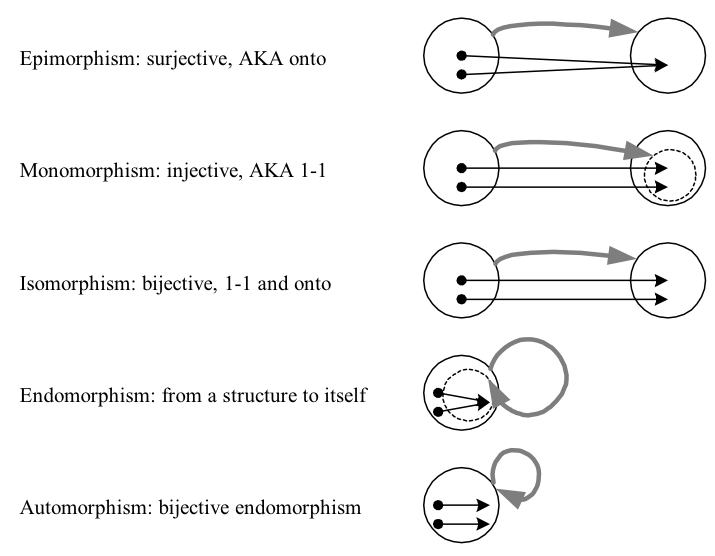
\includegraphics[scale=0.8]{comparisonofmorph}
\caption{Comparison of all types of morphism.}
\end{figure}

\subsubsection{Group Actions}

Group action is a powerful tool for proving theorems for abstract groups, and for unravelling the structure of the groups. This is a method for studying an algebraic object by seeing how it can act on other structures.

\begin{definition}
A \hlt{(left) group action} of a group $G$ on a set $A$ is a map from $G \times A$ to $A$, written as $g \cdot a \ \forall g\in G$ and $a\in A$, satisfying the following properties:
\begin{enumerate}[label=(\roman*)]
\setlength{\itemsep}{0pt}
\item $g_1 \cdot (g_2 \cdot a) = (g_1 g_2) \cdot a$ $\forall g_1, g_,2 \in G$ and $a \in A$, and
\item $1 \cdot a = a$ $\forall a \in A$
\end{enumerate}
A \hlt{right group action} is similarly defined, with group elements on the right of set elements.\\
Hence, for each fixed $g\in G$, we get a map $\sigma_g$ defined by:
\begin{align}
\sigma_g : A &\rightarrow A \nonumber \\
\sigma_g(a) &= g \cdot a \nonumber
\end{align}
\end{definition}

\begin{proposition}{\color{white}space}
\begin{enumerate}[label=(\roman*)]
\setlength{\itemsep}{0pt}
\item For each $g\in G$, $\sigma_g$ is a permutation of $A$, and
\item the map from $G$ to $S_A$ defined by $g \mapsto \sigma_g$ is a homomorphism
\end{enumerate}
\end{proposition}
\begin{proof}{\color{white}space}
\begin{enumerate}[label=(\roman*)]
\setlength{\itemsep}{0pt}
\item To show that $\sigma_g$ is a permutation of $A$, we show that as a set map from $A$ to $A$, it has a $2$-sided inverse $\sigma_{g^{-1}}$. For all $a \in A$: 
\begin{alignat*}{2}
(\sigma_{g^{-1}} \circ \sigma_g)(a) &= \sigma_{g^{-1}}(\sigma_g(a)) \ \ \ && \textnormal{(by definition of function composition)} \\
&= g^{-1} \cdot(g\cdot a) && \textnormal{(by definition of $\sigma_{g^{-1}}$ and $\sigma_g$)} \\
&= (g^{-1} g)\cdot a && \textnormal{(by property (1) of an action)} \\
&= 1 \cdot a = a && \textnormal{(by property (2) of an action)}
\end{alignat*}
Hence, $\sigma_{g^{-1}} \circ \sigma_{g}$ is the identity map from $A$ to $A$, with a $2$-sided inverse. Since $g$ is arbitrary, we may interchange the roles of $g$ and $g^{-1}$ to obtain $\sigma_{g} \circ \sigma_{g^{-1}}$, which is also the identity map on $A$. Hence $\sigma_{g}$ has a $2$-sided inverse, hence is a permutation of $A$.
\item let $\varphi: G \rightarrow S_A$ be defined by $\varphi(g) = \sigma_g$. Note that (i) has shown that $\sigma_g$ is indeed an element of $S_A$. To see that $\varphi$ is a homomorphism, we must prove $\varphi(g_1 g_2) = \varphi(g_1) \circ \varphi(g_2)$. For all $a\in A$:
\begin{alignat*}{2}
\varphi(g_1 g_2)(a) &= \sigma_{g_1 g_2} (a) \ \ \ && \textnormal{(by definition of $\varphi$)} \\
&= (g_1 g_2) \cdot a && \textnormal{(by definition of $\sigma_{g_1 g_2}$)} \\
&= g_1 \cdot (g_2 \cdot a) && \textnormal{(by property (1) of an action)} \\
&= \sigma_{g_1}(\sigma_{g_2} (a)) && \textnormal{(by definition of $\sigma_{g_1}$ and $\sigma_{g_2}$)} \\
&= (\varphi(g_1) \circ \varphi(g_2)) (a) \ \ && \textnormal{(by definition of $\varphi$)}
\end{alignat*}
\end{enumerate}
\end{proof}

\begin{definition}
The \hlt{permutation representation} associated to the group action is the homomorphism from $G$ to $S_A$. Let $\varphi: G \rightarrow S_A$ be any homomorphism from a group $G$ to the symmetric group on a set $A$, then the map $G \times A \mapsto A$ is defined by
\begin{equation}
g \cdot a = \varphi(g)(a) \ \ \forall g\in G, \a \in A \nonumber
\end{equation}
\end{definition}

\begin{definition}
Let $ga=a$ for all $g\in G, a\in A$. Then this is the \hlt{trivial action}, and $G$ is said to \hlt{act trivially} on $A$. The distinct elements of $G$ induce the same permutation on $A$. The associated permutation representation $G\rightarrow S_A$ is the trivial homomorphism which maps every element of $G$ to the identity.
\end{definition}

\begin{definition}
If $G$ acts on a set $B$ and distinct elements of $G$ induce distinct permutations of $B$, then the action is \hlt{faithful}. The associated permutation representation is injective.\\
The \hlt{kernel} of the action $G$ on $B$ is $\ker = \{g \in G \ \vert \ gb = b \ \forall b \in B \}$.
\end{definition}

\subsection{Subgroups}

To study the structure of a group, a basic method is to study quotients of an object (to collapse a group into a smaller group).

\subsubsection{Centralisers, Normalisers, Stabilisers, Kernels}

\begin{definition}
Let $G$ be a group. The subset $H$ of $G$ is a \hlt{subgroup} of $G$ if $H$ is nonempty and $H$ is closed under products and inverses. If $H$ is a subgroup of $G$, this is denoted $H \leq G$.
\end{definition}

\begin{example}{\color{white}space}
\begin{enumerate}[label=(\roman*)]
\setlength{\itemsep}{0pt}
\item $\Z \leq \Q$, and $\Q \leq \R$ with the operation of addition.
\item Any group $G$ has two subgroups: $H = G$, and $H = \{1\}$ (the \hlt{trivial subgroup}).
\item If $H \leq G$ and $K \leq H$, then $H \leq G$ by transitivity property.
\end{enumerate}
\end{example}

\begin{proposition}
\hlt{(The Subgroup Criterion)}
\end{proposition}

\subsection{Quotient Groups, Homomorphisms}

\subsection{Group Actions}

\subsection{Direct and Semidirect Products, Abelian Groups}

This section introduces methods to construct larger groups from smaller ones with direct and semidirect product. This then allow us to completely classify all finite abelian groups with the Fundamental Theorem on Finitely Generated Abelian Groups.

\subsubsection{Direct Products}

\begin{definition}
The \hlt{direct product} $G_1 \times G_2 \times \cdots$ of groups $G_1, G_2, \ldots$ with operations $*_1, *_2, \ldots$ is the set of sequences $(g_1, g_2, \ldots)$ where $g_i \in G_i $, with operation defined component-wise:
\begin{equation}
(g_1, g_2, \ldots) * (h_1, h_2, \ldots) = (g_1 *_1 h_1, g_2 *_2 h_2, \ldots) \nonumber
\end{equation}
\end{definition}

\begin{example}{\color{white}space}
\begin{enumerate}[label=(\roman*)]
\setlength{\itemsep}{0pt}
\item Let $G_i = \R$ for $i = 1,2,\ldots,n$. Then $\R \times \R \times \cdots \times \R$ ($n$-factors) is the Euclidean $n$-space $\R^n$ with vector addition $(a_1, a_2, \ldots, a_n) + (b_1, b_2, \ldots, b_n) = (a_1 + b_1, a_2 + b_2, \ldots, a_n + b_n)$
\item For groups forming direct product, let $G_1 = \Z, G_2 = S_3, G_3 = GL_2(\R)$, where the group operations are addition, composition, and matrix multiplication. Then the operation $G_1 \times G_2 \times G_3$ is defined to be
\begin{equation}
(n,\sigma, \begin{pmatrix}
a & b \\
c & d
\end{pmatrix})
(m,\tau, \begin{pmatrix}
p & q \\
r & s
\end{pmatrix}) =
(n+m,\tau \circ \sigma, \begin{pmatrix}
ap+br & aq+bs \\
cp+dr & cq+ds
\end{pmatrix}) \nonumber
\end{equation}
\end{enumerate}
\end{example}

\begin{proposition}
If $G_1, \ldots, G_n$ are groups, then their direct product is a group of oder $\abs{G_1} \abs{G_2} \cdots \abs{G_n}$. If any $G_i$ is infinite, so is the direct product.
\end{proposition}
\begin{proof}
Let $G = G_1 \times G_2 \times \cdots \times G_n$.\\
The group axioms hold for $G$ since each axiom is a consequence of the fact that the same axiom in Proposition \ref{prop:proofgroupop} holds in each factor $G_i$, and the operation on $G$ is defined component-wise. \\
The identity of $G$ is the $n$-tuple $(1_1, 1_2, \ldots, 1_n)$, where each $1_i$ is the identity of $G_i$.\\
The inverse of $(g_1, g_2, \ldots, g_n)$ is $(g_1^{-1}, g_2^{-1}, \ldots, g_n^{-1})$, where each $g_i^{-1}$ is the inverse of $g_i$ in $G$.\\
Hence the formula for the order of $G$ is clear.
\end{proof}

Rearranging factors of the direct product results in a direct product isomorphic to the original one.

\begin{proposition}
Let $G_1, G_2, \ldots, G_n$ be groups, and let $G = G_1 \times \cdots \times G_n$ be their direct product.
\begin{enumerate}[label=(\roman*)]
\setlength{\itemsep}{0pt}
\item For each fixed $i$, the set of elements of $G$ which have the identity of $G_j$ in the $j^{\textnormal{th}}$ position for all $j \neq i$ and the arbitrary elements of $G_i$ in position $i$ is the subgroup of $G$ isomorphic to $G_i$:
\begin{equation}
G_i \cong \{(1,1,\ldots, 1, g_i, 1, \ldots, 1) \ \vert \ g_i \in G_i\} \textnormal{ (where $g_i$ is at the $i^{\textnormal{th}}$ position)} \nonumber
\end{equation}
If we identify $G_i$ with this subgroup, then $G_i \trianglelefteq G$ and
\begin{equation}
G/G_i \cong G_1 \times \cdots \times G_{i-1} \times G_{i+1} \times \cdots \times G_n \nonumber
\end{equation}
\item For each fixed $i$, define $\pi_i: G \rightarrow G_i$ by
\begin{equation}
\pi_i((g_1 ,g_2, \ldots, g_n)) = g_i \nonumber
\end{equation}
Then $\pi_i$ is a surjective homomorphism with
\begin{align}
\ker{\pi_i} &= \{(g_1, \ldots, g_{i-1}, 1, g_{i+1}, \ldots, g_n)\ \ \vert \ g_j\in G_j \ \forall j\neq i\}\nonumber \\
&\cong G_1 \times \cdots \times G_{i-1} \times G_{i+1} \times \cdots \times G_n \nonumber
\end{align}
where $1$ appears at position $i$. 
\item Under the identifications in part (i), if $x \in G$ and $y \in G_j$ for some $i\neq j$, then $xy = yx$
\end{enumerate}
\end{proposition}

\subsection{Further Topics in Group Theory}

\subsubsection{$p$-groups, Nilpotent Groups, Solvable Groups}


